\documentclass{article}

% Language setting
% Replace `english' with e.g. `spanish' to change the document language
\usepackage[english]{babel}

% Set page size and margins
% Replace `letterpaper' with `a4paper' for UK/EU standard size
\usepackage[letterpaper,top=2cm,bottom=2cm,left=3cm,right=3cm,marginparwidth=1.75cm]{geometry}

% Useful packages
\usepackage{amsmath}
\usepackage{graphicx}
\usepackage{float}
\usepackage[clean]{svg}
\usepackage[colorlinks=true, allcolors=blue]{hyperref}
\usepackage{multirow,tabularx}

\title{RockX Liquid Staking Explained}
\author{RockX Team}

\begin{document}
\maketitle

\begin{abstract}
Staking, a cryptoeconomic primitive that allows participants to earn yield in exchange for locking tokens, has taken center stage over the past two years. Under Proof of Stake consensus mechanism, instead of using computational power, validators lock (“stake”) a certain amount of the network’s native cryptoasset as collateral to create new blocks. In return, they earn inflationary rewards and transaction fees.
\end{abstract}

\section{Introduction}

\subsection{What is Proof of Stake?}

Proof of Stake is the consensus protocol utilised in Ethereum 2.0 (ETH2). The consensus protocol helps everyone to know what transactions have been processed and in what order, which is known as validation.

ETH2 currently has a Proof of Stake (PoS) chain called the Beacon Chain, which is faster, more energy efficient and more decentralised than the current consensus protocol Ethereum is utilising (Proof of Work). Users deposit ETH and provide an Ethereum node to perform the required validation. As a reward for providing the node, the Beacon Chain gives node operators additional ETH on top of their deposits. These rewards are minted in return for helping secure the network.

\subsection{What is liquid staking?}

It is clear that PoS chains will be an integral part of the future of crypto, and become the foundation layer of which DeFi and metaverses will be built on.

However, PoS comes with some drawbacks for those wanting to participate directly as validators:

It requires technical know-how to set up and operate
32ETH is a significant barrier for regular token holders to participate in POS validation
Staked tokens are locked up and become illiquid assets
In order to solve these issues, liquid staking protocols were born. Liquid staking abstracts the depositing of tokens from running a validator node.

In exchange for their tokens, depositors receive a representative (uniETH) token from the protocol which is a claim on the tokens they have staked.

\subsection{What is uniETH?}

uniETH represents the staked ETH plus all future staking rewards. uniETH does not grow in quantity over time but instead, grows in value, i.e. 1 uniETH becomes worth increasingly more than 1 ETH.

\subsection{What should I stake with RockX instead of staking directly to ETH2?}

RockX removes several drawbacks that exist with Proof of Stake on ETH2.

The Beacon Chain requires a minimum deposit of at least 32 ETH. RockX will allow anyone to earn the reward on any amount of ETH deposited with us.

When depositing ETH on the Beacon Chain, users are required to have technical knowledge of interacting with smart contracts. RockX handles all interaction with the Beacon Chain in our users’ place. The Beacon Chain will also require users who make deposits to be technically proficient at running Ethereum nodes 24/7, at the same time keeping that node online and secure. RockX provides this service in our users’ place.

As ETH2 is being rolled out in several phases. We are currently in phase 1, the merge, and depositing now means your deposit is locked until phase 2 arrives, which could very well still be a long time away. With RockX you instantly get uniETH when depositing and do not need to be locked with us. It can be traded, sold or held at any time, which provides our users with liquidity on their staked ETH.

\subsection{What is the staking period for uniETH?}
The staking period to redeem the underlying ETH on uniETH will only be confirmed till ETH2 goes into phase 2. However, you will receive uniETH when you deposit and it will still gain staking rewards over time in terms of the token value. uniETH can also be sold and traded on various DEXs and CEXs if there is liquidity available for the trade.

\subsection{What is the minimum deposit?}
RockX gives everyone the opportunity to earn rewards on any amount of ETH, as we do not have a minimum. We do recommend a deposit of at least 0.01ETH to make your transaction worthwhile. When you stake ETH, you will receive uniETH, which gains rewards over time based on the performance of our nodes on the Beacon Chain.

\subsection{What is the maximum deposit?}
There is no limit on the amount of ETH you can stake with RockX on ETH2. The more ETH, the more rewards you will be receiving.

\section{RockX uniETH staking algorithm}

\subsection{Terminology}
\begin{description}
   \item[ETH] $1\cdot ETH \equiv 10^{18}$
   \item[TotalSupply] current total supply of uniETH.
   \item[TotalStaked] total ethers staked to validators.
   \item[TotalDebts] total unpaid debts, generated from \textbf{redeemFromValidators()}, awaiting to be paid by turning off validators and initiates debt clearance procedure.
   \item[TotalPending] pending ethers to be staked.
   \item[RewardDebts] the remaining ethers from debt clearance procedure.
   \item[AccountedUserRevenue] overall net revenue which belongs to all uniETH holders.
   \item[ReportedValidators] latest reported active validators.
   \item[ReportedValidatorBalance] latest reported overall balance of active validator.
   \item[RecentEthersMoved] the amount this contract receives recently from validators.
   \item[CurrentReserve] overall assets under management, given as:
   \[CurrentReserve = TotalPending + TotalStaked + AccountedUserRevenue - TotalDebts - RewardDebts\]
   \item[Exchange Ratio] Defined as symbol $\rho$ of uniETH to ETH, given as: 
    \[\rho = \frac{TotalSupply}{CurrentReserve} , \{normally: \rho \leq 1.0\} \]
   \item[managerFeeShare] share of the manager fee, represented as 1 in 1000, managerFeeShare $\in[0,1000]$ 
\end{description}

\newtheorem{theorem}{Theorem}[section]
\newtheorem{corollary}{Corollary}[theorem]
\newtheorem{lemma}[theorem]{Lemma}

\subsection{The liquid staking algorithm explained}
In this section, we'll explain the details of liquid staking below from a user's perspective.

\subsection{Stake ethers to mint uniETH}
A user calls function \textbf{mint()} with a specific amount of \textbf{ethersToStake} ethers to mint \textbf{uniETH}, in each function call, we have:

\begin{theorem}
\label{Mint}
\[minted_{uniETH} := \rho \cdot ethersToStake \]
\[TotalSupply = TotalSupply^{\prime} + minted_{uniETH} \]
\[TotalPending = TotalPending^{\prime} + ethersToStake\]
\end{theorem}

Users receives $minted_{uniETH}$ token of uniETH  if \textbf{mint()} succeeds. \textbf{uniETH} is a standard \textbf{ERC-20} compliant contract issued by RockX staking contract only, can it can be exchanged at will, uniETH can also be traded on \textbf{DEX}s for liquidation other than redeeming from official contract as long as there are sufficient liquidity on DEXs.

\subsection{Initiating delegation into ETH2 offical contract}
At any time \textbf{TotalPending} has more than $32 ethers$, the contract manager can call \textbf{stake()} function to stake the ethers into Ethereum 2.0 staking contract, then \textbf{TotalPending} moves to \textbf{TotalStaked} and keeps \textbf{TotalPending} less than $32 ethers$, we calculate the changes as followings:

\begin{lemma}
\[ethersToStake := \lfloor\frac{TotalPending^{\prime}}{32ETH}\rfloor \cdot 32ETH\]
\end{lemma}

The ethers to delegate to ETH2 official contract is rounded to $N\cdot 32ETH$ as above, then:

\begin{theorem}
\label{Stake}
\[TotalPending = TotalPending^{\prime} - ethersToStake \]
\[TotalStaked = TotalStaked^{\prime} + ethersToStake \]
\end{theorem}

The timing for calling stake() function mainly considers to maximize capital efficiency, if we stake too soon, the cost for running a single validator is way too expensive, on the contrary, if we stake too late, the staked ethers does not generate rewards during the period before ethers staked to official ETH2 staking contract, so we have built an off-chain program to provide a seamless and comprehensive solution for staking, allowing maximum capital efficiency on assets while earning cryptonative yields.

\subsection{Redeeming staked ethers from official RockX smart contract}
Users call function \textbf{redeemFromValidators()} with a specific amount of \textbf{ethersToRedeem} ethers expected to redeem, the amount uniETH to be burnt is exactly to $N\cdot 32ETH$ worth of uniETH, then we have:
\begin{theorem}
\label{Redeem}
\[burned_{uniETH} := \rho \cdot ethersToRedeem \]
\[TotalSupply = TotalSupply^{\prime} - burned_{uniETH} \]
\[TotalDebts = TotalDebts^{\prime} + ethersToRedeem\]
\end{theorem}
Redeeming(or Unstaking) works as by turning off validators, to wait until the validators to be offline and return the staked ethers to the contract. So it's a time-consuming asynchronous process. The benefit from redeeming directly from this contract is that, there's no slippage as in CEX or DEX, but you have to be patient. Once the ethers returned, you'll be notified to claim the ethers.

Note: redeeming function will only be available after ETH2.0 merged.

\subsection{How ethers returns to this contract from validators? }
\label{sectionAccounting}

The way the withdrawals implementation is currently, withdrawals are not like normal transactions, and are instead system level transactions that update an account's balance without a transaction in or out. In our contract implementation, we use \textbf{accountedBalance} to track the in and out of the ethers, and compare \textbf{accountedBalance} with \textbf{this.balance}, the difference is the ethers reward returned from validators. We utilize variable \textbf{RecentEthersMoved} to track this difference:

\[RecentEthersMoved = accountedBalance - this.balance\]

Ethers moves from contract to validators, or vice versa, we can assume: \textbf{RecentEthersMoved} is the ethers moved from ${validators}\Longrightarrow{contract}$.

\subsection{Stopping validators for debt clearance}
Whenever a validator stopped by a node operator, the ethers are supposed to return to this contract by the setting of \textsc{withdrawal\_credentials}, once the ethers returned, the oracle calls \textbf{validatorStopped()} function, along with the following parameters:
\begin{description}
\item[valueStopped] The ethers sent-back from validators to the liquid staking contract.
\item[validatorStopped] The count of stopped validators.
\end{description}
Suppose:

\[valueStopped \geq amountUnstaked \]
and meanwhile, \textbf{RecentEthersMoved} will be updated as explained in section:\ref{sectionAccounting}.
\[RecentEthersMoved = RecentEthersMoved^{\prime} + valueStopped\]

If we do not have \textbf{slashing}, then we have:
\begin{lemma}
\[amountUnstaked := 32 ETH \cdot validatorStopped\]
\[incrRewardDebt := valueStopped - amountUnstaked\]
\end{lemma}

then, we use these 2 varaibles above to update the following variables:
\begin{theorem}
\label{validatorStopped}
\[RewardDebts = RewardDebt^{\prime} + incrRewardDebt\]
\[TotalPending = TotalPending^{\prime} + Max(0, amountUnstaked - TotalDebts) + incrRewardDebt\]
\[TotalStaked = TotalStaked^{\prime} -  amountUnstaked \]
\end{theorem}

\subsection{Calculating rewards}
An oracle service will push overall alive validators balance periodically, there're 2 things \textbf{pushBeacon()} do to calculate the reward:

\subsubsection{Adjusting reward base}
Firstly, pushBeacon will check if there is new validator alive, the reward base will be aligned to the new staked value plus previously reported validators balance, the \textbf{reward base} is the defined as the base-point to check for balance increasement, given:
\begin{description}
\item[aliveValidator] The count of validators alive
\end{description}
we have:
\begin{theorem}
\label{pushBeacon}
\[RewardBase = ReportedValidatorBalance + Max(0, aliveValidator - ReportedValidators) \cdot  32 ETH\]
\end{theorem}

\subsubsection{Reward distribution}
Secondly, revenue will be accumulated as followings if there's any. Normally ethers will either stays in contract or validators, the overall assets under management is:
\[TVL := ethersInContract + ethersInValidators\]

During calculation of rewards changes, we only consider the balance change in alive validators, we can assume that, if:
\[aliveBalance + RecentEthersMoved \geq RewardBase\]

then rewards has generated, we formalize the formula as below, given:

\begin{description}
\item[aliveBalance] The balance of current alive validators
\end{description}
we have:

\begin{theorem}
\label{calcReward}
\[r := Max(0, aliveBalance + RecentEthersMoved - RewardBase)\]
\[AccountedUserRevenue = AccountedUserRevenue^{\prime} + r \cdot \frac{(1000 - managerFeeShare)}{1000}\]
\[RecentEthersMoved = 0\]
\[ReportedValidators = aliveValidator\]
\[ReportedValidatorBalance = aliveBalance\]
\end{theorem}

As \textbf{RecentEthersMoved} will only be counted during reward distribution, the variable will be reset to 0 at the end of each \textbf{pushBeacon()} call. The exchange ratio will go down by the change of \textbf{AccountedUserRevenue}.

\subsection{Slashing}
Nobody expects slashing, but what if it happens, under such rare case, users will face a sudden change of \textbf{exchange ratio}, actually we made a tiny modification to handle this situation in \textbf{pushBeacon()} and \textbf{validatorSlashedStop()}

\subsubsection{Slashing notification in validatorSlashedStop()}
Given:
\begin{description}
\item[remainingEthers] The ethers left after slashing
\item[slashedAmount] The ethers slashed
\item[slashedValidators] The count of slashed validators.
\end{description}
we have:
\begin{theorem}
\[TotalPending = TotalPending^{\prime} + remainingEthers \]
\[TotalStaked = TotalStaked^{\prime} - 32 ETH \cdot slashedValidators \]
\[RecentSlashed = RecentSlashed^{\prime} +  slashedAmount \];
\end{theorem}

\subsubsection{Modification of rewards calculation in pushBeacon()}
\begin{theorem}
\[r := Max(0, aliveBalance + RecentEthersMoved + RecentSlashed - RewardBase)\]
\[AccountedUserRevenue = AccountedUserRevenue^{\prime} + r \cdot \frac{(1000 - managerFeeShare)}{1000}\]
\[RecentEthersMoved = 0\]
\[RecentSlashed = 0\]
\[ReportedValidators = aliveValidator\]
\[ReportedValidatorBalance = aliveBalance\]
\end{theorem}

\subsection{Understanding rewards via balance sheet}
\begin{table}[!ht]
    \centering
    \begin{tabular}{p{0.2\linewidth} | p{0.3\linewidth}| p{0.1\linewidth}| p{0.2\linewidth}| p{0.2\linewidth}}
    \hline
        \textbf{Initial Stage}:  & ~ & ~ & ~ & ~ \\ \hline
        User A Stakes 32 ETH & \textbf{ASSETS} & ETH & \textbf{LIABILITY} & uniETH \\ \hline
        ~ & \textbf{User A Deposit} & 32 & User A uniETH & 32 \\ \hline
        ~ & Total Assets & 32 & Total Liability & 32 \\ \hline
        ~ & SwapRatio & ~ & ~ & 1 \\ \hline
        \multicolumn{5}{c}{} \\ \hline
        \textbf{Stage 1}:  & ~ & ~ & ~ & ~ \\ \hline
        Got 0.32 ETH Rewards & \textbf{ASSETS} & ETH & \textbf{LIABILITY} & uniETH \\ \hline
        ~ & User A Deposit & 32 & User A uniETH & 32 \\ \hline
        ~ & \textbf{Mining Rewards} & 0.32 & ~ & ~ \\ \hline
        ~ & Total Assets & 32.32 & Total Liability & 32 \\ \hline
        ~ & SwapRatio & ~ & ~ & 1.01 \\ \hline
        \multicolumn{5}{c}{} \\ \hline
        \textbf{Stage 2}:  & ~ & ~ & ~ & ~ \\ \hline
        User B Stakes 64 ETH & \textbf{ASSETS} & ETH & \textbf{LIABILITY} & uniETH \\ \hline
        ~ & User A Deposit & 32 & User A uniETH & 32 \\ \hline
        ~ & \textbf{User B Deposit} & 64 & User B uniETH & 63.36633663 \\ \hline
        ~ & Mining Rewards & 0.32 & ~ & ~ \\ \hline
        ~ & Total Assets & 96.32 & Total Liability & 95.36633663 \\ \hline
        ~ & SwapRatio & ~ & ~ & 1.01 \\ \hline
        \multicolumn{5}{c}{} \\ \hline
        \textbf{Stage 3}: & ~ & ~ & ~ & ~ \\ \hline
        User B transfer 32 uniETH to User C & \textbf{ASSETS} & ETH & \textbf{LIABILITY} & uniETH \\ \hline
        ~ & ~ & ~ & User A uniETH & 32 \\ \hline
        ~ & ~ & ~ & User B uniETH & 31.36633663 \\ \hline
        ~ & ~ & ~ & \textbf{User C uniETH} & 32 \\ \hline
        ~ & Total Assets & 96.32 & Total Liability & 95.36633663 \\ \hline
        ~ & SwapRatio & ~ & ~ & 1.01 \\ \hline
        \multicolumn{5}{c}{} \\ \hline
        \textbf{Stage 4}: & ~ & ~ & ~ & ~ \\ \hline
          User A unstakes equivalent 32 ETH value of uniETH & \textbf{ASSETS} & ETH & \textbf{LIABILITY} & uniETH \\ \hline
        ~ & Before Redeeming & 96.32 & User A uniETH & 32 \\ \hline
        ~ & ~ & ~ & User B uniETH & 31.36633663 \\ \hline
        ~ & ~ & ~ & User C uniETH & 32 \\ \hline
        ~ & \textbf{User A Redeems} & -32 & User A Burned & -31.68316832 \\ \hline
        ~ & Total Assets & 64.32 & Total Liability & 63.68316831 \\ \hline
        ~ & SwapRatio & ~ & ~ & 1.01 \\ \hline
    \end{tabular}
    \caption{RockX ETH2 Liquid Staking Balance Sheet}
\end{table}

\section{RockX liquid staking architecture}
\begin{figure}[H]
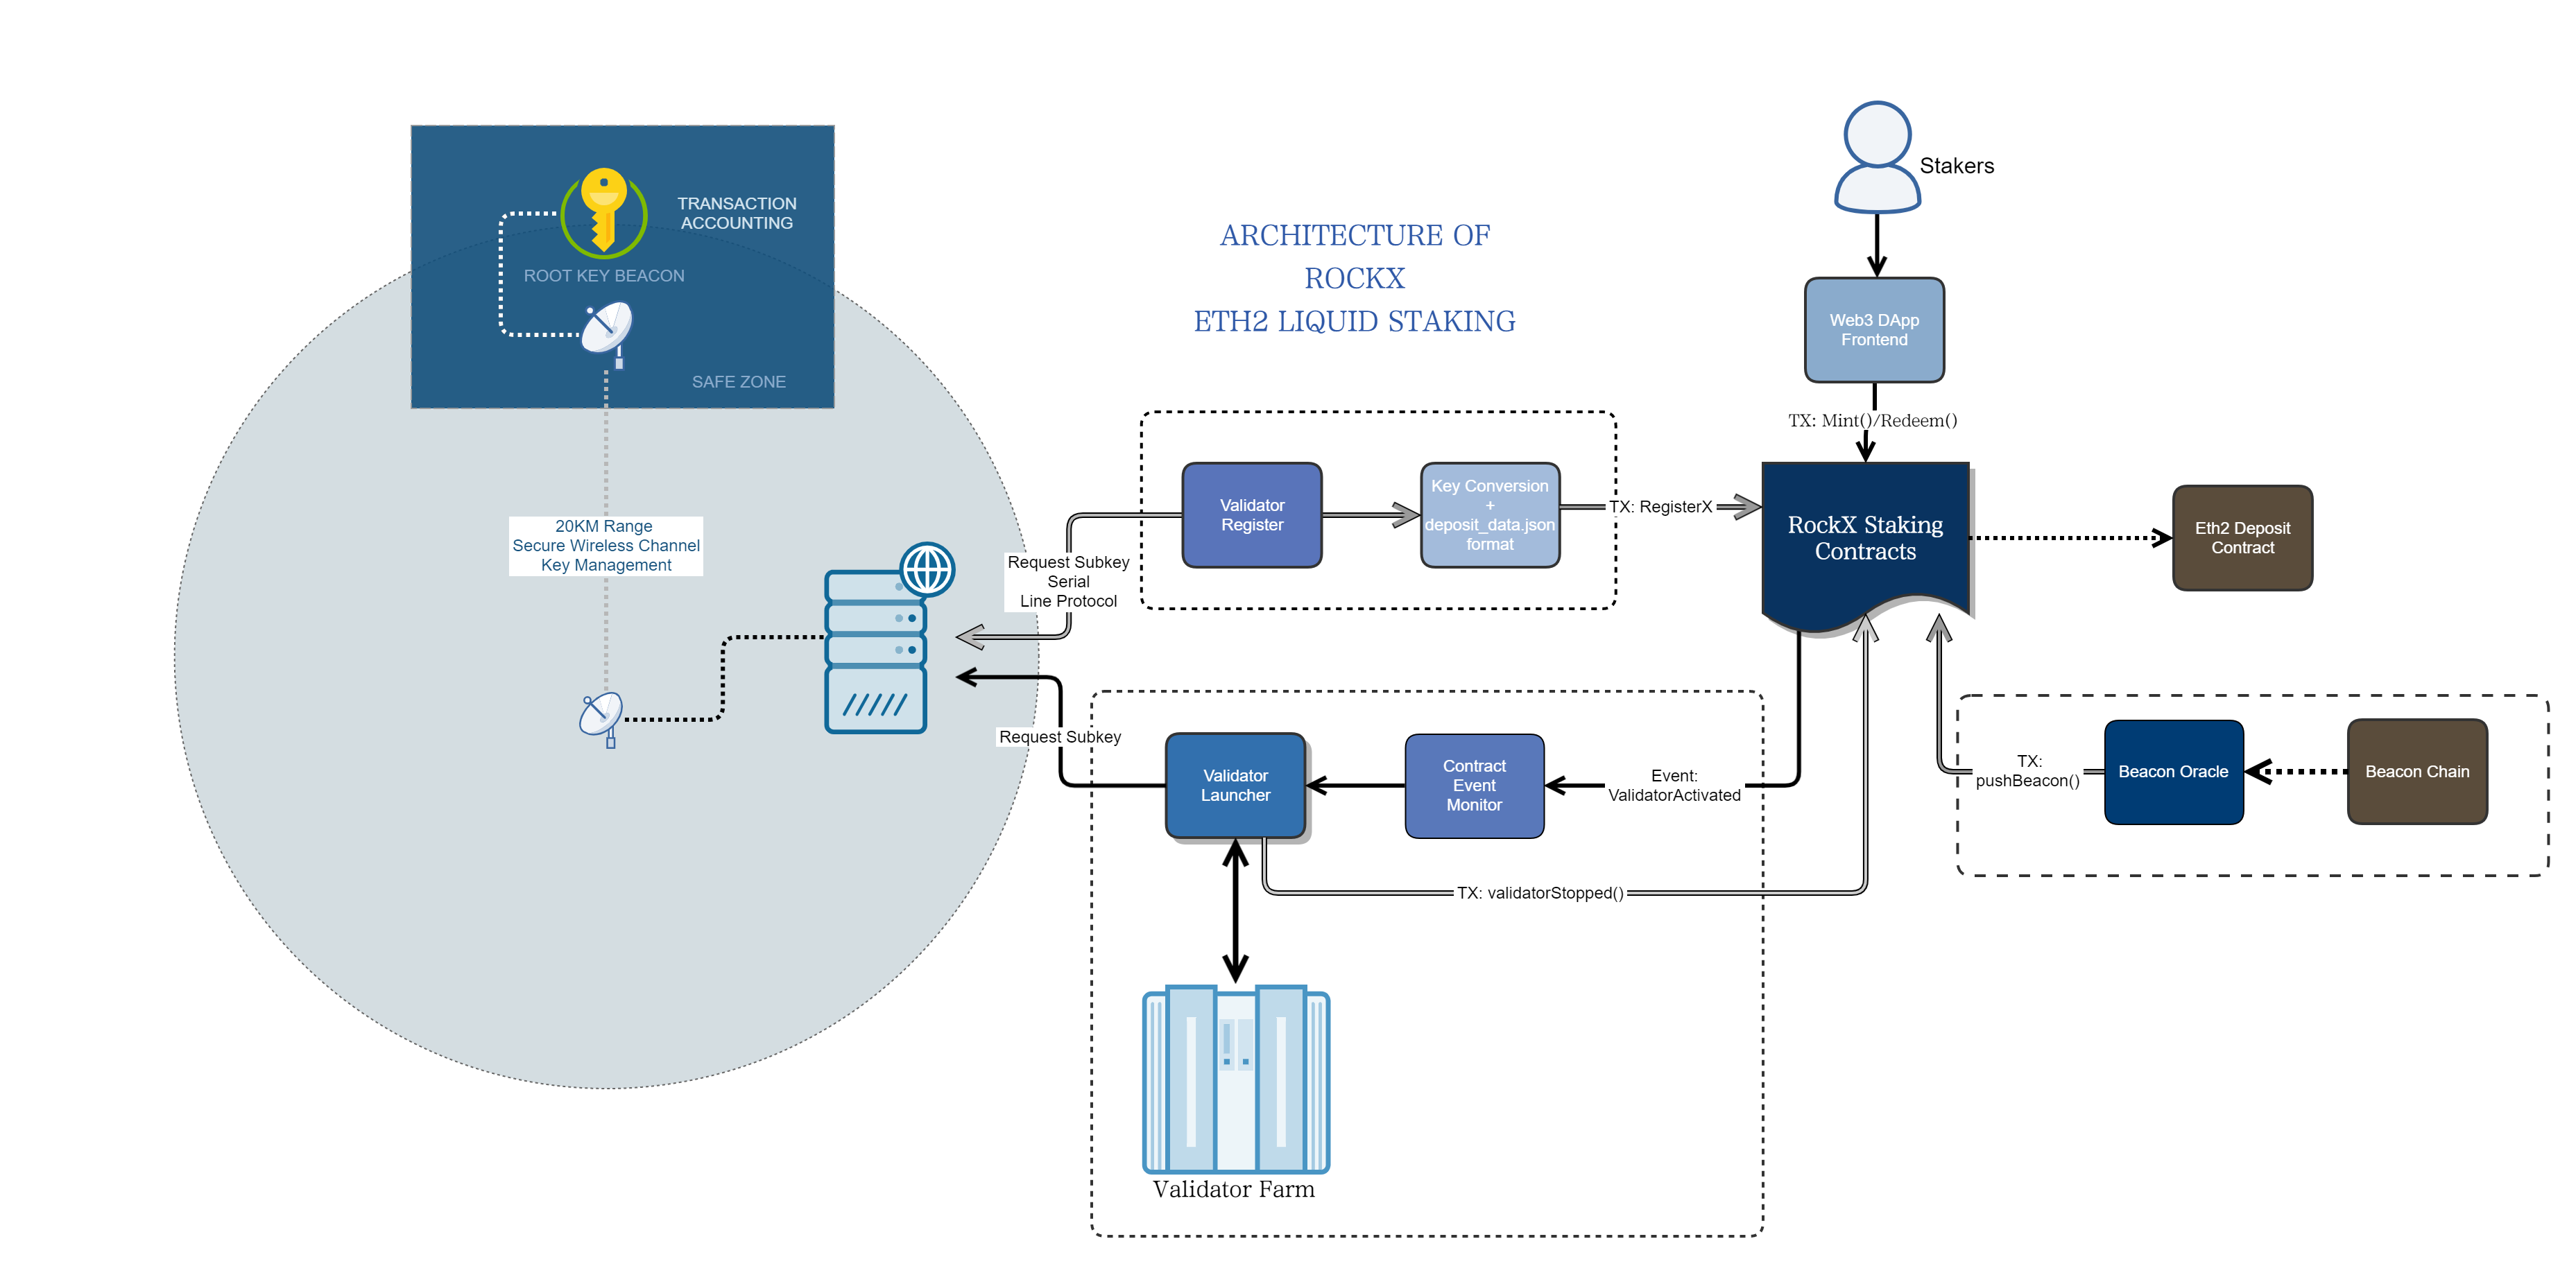
\includegraphics[scale=0.1]{arch.png}
\end{figure}

\section{DAO Governance}
(TBD)
\section{Conclusion}
(TBD)

\end{document}